\newpage
{\bfseries МРНТИ 71.37.01}
\hfill {\bfseries \href{https://doi.org/10.58805/kazutb.v.2.23-405}{https://doi.org/10.58805/kazutb.v.2.23-405}}

\sectionwithauthors{Ж. Бидахмет, А.Р. Исаев}{КҮРДЕЛІ БИЗНЕС ПРОЦЕСТІ БАСҚАРУДЫҢ АҚПАРАТТЫҚ ЖҮЙЕСІ МЕН
АЙМАҚТЫҚ ДАМУДЫҢ КӨП НҰСҚАЛЫ РЕГРЕССИЯЛЫҚ ТАЛДАУЫ}

\begin{center}
{\bfseries Ж. Бидахмет, А.Р. Исаев\envelope}

\textsuperscript{1}әл-Фараби атындағы Қазақ ұлттық университеті, Алматы,
Қазақстан

\envelope Корреспондент-автор: aydarisaev@mail.ru
\end{center}

Қазіргі таңда, әлемде бізді тұтас компьютерлік инновациялар, түрлі
бағдарламалық құралдар қоршап тұр. Қызметтің барлық салаларында
ақпараттық технологиялар қолданылады. Сол сияқты,күнделікті өмірімізде
әртүрлі курорттар, демалыс және ойын-сауық орындары көбейіп келеді. Әр
жолы туристерді таң қалдыру қиынырақ, керісінше, көптеген адамдар,
сауалнамалар мен зерттеулер көрсеткендей, адамның "өркениетті аяғы"
жетпеген жердің бұрыштарына, қалалардан алыс, табиғатқа, шулы көліктер
жоқ жерде, адамдар көп емес жерде тіпті, табиғат-ананың сұлулығынан
ләззат алып саяхаттауды жөн көреді. Ал, дәл осындай жерлер кең байтақ
Қазақстанда өте көп десе де болады.

Қазақстанда туризмді дамыту үшін бірінші кезекте \emph{Ақпараттық
өрісті} дамыту қажет. Қазақстандағы туристік ақпараттық жүйелер (АЖ)
бірқатар проблемаларды бастан кешіруде, мысалы: бір типтілік,
консервативтілік және т. б.

Бұл жұмыста ақпараттық туризммен байланысты бірқатар мәселелердің
сипаттамасы, сондай-ақ шешімнің бір моделі ұсынылады. Негізгі мақсат --
көп нұсқалы регрессия әдістерін қолдана отырып, туризмнің экономикалық
өсуге, жұмыспен қамтуға және әлеуметтік инфрақұрылымның дамуына қалай
әсер ететінін сандық талдау. Деректер әртүрлі аймақтық көздерден, соның
ішінде Қазақстан Статистика агенттігінен, туризм департаментінің
жазбаларынан және 2019 және 2022 жылдар аралығында жергілікті бизнес пен
туристермен жүргізілген сауалнамалардан жиналды. Талдау туризммен
байланысты қызмет пен әлеуметтік-экономикалық нәтижелер арасындағы
қарым-қатынасты анықтау үшін көптеген регрессиялық модельдерді
пайдаланды. Зерттеу туризмнің әсерін күшейтетін негізгі факторларды,
соның ішінде инфрақұрылымды жақсартуды, қызмет көрсету сапасына
инвестицияны және тұрақты тәжірибеге бағытталған стратегиялық
маркетингті анықтайды. Бұл зерттеу басқа контекстердегі ұқсас
зерттеулердің үлгісін ұсына отырып, аз танымал аймақтардағы туризмнің
трансформациялық күшін тереңірек түсінуге ықпал етеді.

{\bfseries Түйін сөздер:} ақпараттық жүйелер, сандық талдау, сыртқы
факторлар, регрессиялық талдау, инфрақұрылымдық инвестиция,
технологиялық инновациялар, аймақтық даму.

\begin{center}
{\large\bfseries МНОГОФАКТОРНЫЙ РЕГРЕССИОННЫЙ АНАЛИЗ СЛОЖНОЙ ИНФОРМАЦИОННОЙ
СИСТЕМЫ УПРАВЛЕНИЯ БИЗНЕС-ПРОЦЕССАМИ И РЕГИОНАЛЬНОГО РАЗВИТИЯ}

{\bfseries Ж. Бидахмет, А.Р. Исаев\envelope}

\textsuperscript{1}Казахский национальный университет имени аль-Фараби,
Алматы, Казахстан,

е-mail: aydarisaev@mail.ru
\end{center}

Сегодня, в мире, нас окружают целые компьютерные инновации, различные
программные средства. Во всех сферах деятельности используются
информационные технологии. Точно так же в нашей повседневной жизни
появляется все больше различных курортов, курортов и развлекательных
заведений. С каждым разом туристов удивлять сложнее, наоборот, многие,
как показывают опросы и исследования, предпочитают путешествовать,
наслаждаясь красотой матери-природы, в уголки Земли, куда не доходят
"цивилизованные ноги" человека, вдали от городов, на природу, там, где
нет шумных машин, там, где не так много людей. А таких мест в огромном
Казахстане очень много.

Для развития туризма в Казахстане необходимо в первую очередь развивать
информационное поле. Туристические информационные системы (ИС) в
Казахстане испытывают ряд проблем, таких как: однотипность,
консервативность и др.

В данной работе предлагается описание ряда проблем, связанных с
информационным туризмом, а также одна модель решения. Основная цель
состоит в количественном анализе того, как туризм влияет на
экономический рост, занятость и развитие социальной инфраструктуры с
использованием методов многомерной регрессии. Данные были собраны из
различных региональных источников, включая статистическое агентство
Казахстана, отчеты департамента туризма и опросы местных предприятий и
туристов в период с 2019 по 2022 год. В анализе использовалось множество
регрессионных моделей для определения взаимосвязи между деятельностью,
связанной с туризмом, и социально-экономическими результатами.
Исследование определяет ключевые факторы, которые усиливают влияние
туризма, включая улучшение инфраструктуры, инвестиции в качество услуг и
стратегический маркетинг, ориентированный на устойчивые методы. Это
исследование способствует более глубокому пониманию преобразующей силы
туризма в менее известных регионах, предлагая модель аналогичных
исследований в других контекстах.

{\bfseries Ключевые слова:} информационные системы, количественный анализ,
внешние факторы, регрессионный анализ, инвестиции в инфраструктуру,
технологические инновации, региональное развитие.

\begin{center}
{\large\bfseries MULTIFACTORIAL REGRESSION ANALYSIS OF A COMPLEX INFORMATION
SYSTEM FOR BUSINESS PROCESS MANAGEMENT AND REGIONAL DEVELOPMENTRESSION
ANALYSIS OF REGIONAL DEVELOPMENT}

{\bfseries Zh. Bidakhmet, А.R. Isaev\envelope}

\textsuperscript{1}Al-Farabi Kazakh National University, Almaty,
Kazakhstan,

е-mail: aydarisaev@mail.ru
\end{center}

Today, in the world, we are surrounded by whole computer innovations,
various software tools. Information technologies are used in all fields
of activity. Similarly, there are more and more different resorts,
resorts and entertainment venues in our daily lives. It is more
difficult to surprise tourists every time, on the contrary, many, as
surveys and studies show, prefer to travel, enjoying the beauty of
mother nature, to corners of the Earth where "civilized feet" of man do
not reach, away from cities, to nature, where there are no noisy cars,
where there are not so many people. And there are a lot of such places
in the vast Kazakhstan.

For the development of tourism in Kazakhstan, it is necessary first of
all to develop the information field. Tourism information systems (IS)
in Kazakhstan are experiencing a number of problems, such as:
uniformity, conservatism, etc.

This paper offers a description of a number of problems related to
information tourism, as well as one solution model. The main objective
is to quantify how tourism affects economic growth, employment and
social infrastructure development using multidimensional regression
methods. The data was collected from various regional sources, including
the Statistical Agency of Kazakhstan, reports from the Department of
Tourism and surveys of local businesses and tourists between 2019 and
2022. The analysis used a variety of regression models to determine the
relationship between tourism-related activities and socio-economic
outcomes. The study identifies key factors that enhance the impact of
tourism, including infrastructure improvements, investments in quality
services, and strategic marketing focused on sustainable practices. This
study contributes to a deeper understanding of the transformative power
of tourism in lesser-known regions by offering a model of similar
research in other contexts.

{\bfseries Keywords:} information systems, quantitative analysis, external
factors, regression analysis, infrastructure

investments, technological
innovations, regional development.

\begin{multicols}{2}
{\bfseries Кіріспе.} Қазіргі таңда ақпараттық технология күннен күнге
қарқынды даму үстінде. Біздің технологиялар қарқынды дамып жатқан
әлемде, компаниялардың бәсекелестік нарықта өз орнын ойып алудың басты
құралы -- ақпарат болып саналады. Ақпарат қазіргі экономикалық қызметте
есептеме басы болып табылады және де бұл кездейсоқтық емес. Ақпараттық
технологиялар заманауи өркенниеттің инфроқұрылымының барлық сыни
элементтерін басқарудың мәнін құрайды. Жаһандық экономиканың негізгі
саласы болып табылатын туризм индустриясы әлеуметтік-экономикалық
факторлардың, технологиялық жетістіктердің және жаһандық дағдарыстардың
әсерінен қалыптасатын күрделі қиындықтар мен мүмкіндіктерге тап болып
отыр. Пандемияның жаһандық туризмге трансформациялық әсерін бағалайтын
Госслинг, Скотт және Холл (2020) талдаған COVID-19 пандемиясы саланың
осалдығын және стратегиялық тұрақтылық қажеттілігін атап өтті {[}1{]}.
Бұл іргелі өзгеріс тұрақтылық пен бейімделгіштікке баса назар аудара
отырып, туристік тәжірибелерді қайта бағалауды қажет етеді. Әлемдегi
тенденцияларды ескере отырып, Қазақстанда да бұл мәселелер өзектi
проблемалардың бiреуi болып тұр деп айтуға болады.

Технологиялық инновациялар туризм индустриясында төңкеріс жасауды
жалғастыруда. Ли және т.б. (2019) туристерге нақты уақытта, теңшелген
қызметтерді ұсына отырып, туризмді басқаруды айтарлықтай жақсартатын
смарт технологиялардың интеграциясын талқылайды {[}2{]}. Сонымен қатар,
Сигала (2018) пәнаралық тәсілдер арқылы туризмді қайта құрудағы рөлін
атап көрсете отырып, жаңа технологиялардың бұзушы әлеуетін қарастырады
{[}3{]}.

Тұрақтылық туризмді дамытудың негізі болып қала береді. Budeanu және
т.б. (2016) экологиялық, экономикалық және әлеуметтік факторлар
арасындағы тепе-теңдікті жақтап, туризмдегі тұрақты тәжірибені енгізудің
қос қиындықтары мен мүмкіндіктерін зерттейді {[}4{]}. Сол сияқты,
Хиггинс-Десбиоллес (2018) әсіресе пандемия сияқты жаһандық
сын-қатерлерге жауап ретінде әлеуметтік және экологиялық әділеттілікті
насихаттайтын туристік модельді талап етеді {[}5{]}.

Экономикалық ойлар да бірдей маңызды. Брида, Кортес-Джименез, және
Пулина (2016) туризмнің әртүрлі аймақтардағы экономикалық әсері туралы
түсініктерді ұсына отырып, туризмге негізделген өсу гипотезасының
дұрыстығын қарастырады {[}6{]}.

Туризм динамикасын түсінуде теориялық негіздер де маңызды рөл атқарады.
Батлердің (1980) туристік аймақтың өмірлік циклі концепциясы туристік
бағыттардың эволюциялық кезеңдерін және олардың ресурстарды басқарудағы
салдарын зерттеуге теориялық объективті ұсынады {[}7{]}. Бұл модель осы
саладағы практикалық және эмпирикалық зерттеулерді толықтыратын іргелі
теорияны ұсынады.

{\bfseries Материалдар мен әдістер.} Күрделі жүйелер математикалық
модельдер қойылу әдістерін және оларды зерттеу тәсілдері --жаңа ғылыми
60 жылдары пайда болған. 21 --шы ғасыр заманы -- күрделі жүйелер
теориясы. Күрделі жүйелер элементтерін математикалық сипаттау үшін
функциялар теориясын, заманауи алгебраны және функционалдық анализді
пайдаланады. Күрделі зерттеуді әдетте тиімділік, сенімділік,
қауіпсіздік, басқару сапасы және басқа да күрделі жүйелердің маңызды
қасиеттері көрсеткіштері болып табылатын функционалдық сипаттамаларын
бағалаудан бастайды.Кез --келген күрделі жүйенің түйістіру сұлбасы бұл
предикаттар жиынтығы ретінде анықталады, оның элементтерінің көптеген
кірістер мен шығыстарға бөлінген, алайда күрделі жүйе құрылымын зерттеу
үшін математикалық логика және графтар теориясы аппаратын пайдаланады.
Құрылымдық анализ тәсілі күрделі жүйеден белгілі бір байланыста болған
жүйе ішіндегі жүйе тізбектерін бөліп алуға мүмкіндік береді, және
күрделі жүйені жақсы зерттелген типтік құрылымы бар объектілер жиынтығы
ретінде біле аламыз.

Жалпы бизнес процесті жобалау барысында да қолданатын жүйе күрделі жүйе
болып табылады. Бұл зерттеуге арналған деректер туризмнің әсерін
жан-жақты көрсету үшін бірнеше билік органдарынан алынды. 2010-2020
жылдар аралығында келушілер статистикасы, кіріс және маусымдық туризм
үлгілері Солтүстік Қазақстан облыстық туризм басқармасымен ұсынылды.
ЖІӨ~(жалпы ішкі өнім), жұмыспен қамту деңгейі және табыс деңгейі сияқты
экономикалық көрсеткіштер Қазақстанның Ұлттық статистика басқармасынан
алынды {[}8{]}. Жергілікті үкімет көздерінен алынған есептер көлік,
қонақжайлылық және коммуналдық инфрақұрылымдағы өзгерістер туралы
мәліметтерді қамтамасыз етті {[}9{]}. Сонымен қатар, білім беру,
денсаулық сақтаудың қолжетімділігі және өмір сапасы көрсеткіштеріне
қатысты көрсеткіштер Қазақстанның денсаулық сақтау және білім
министрлігінен алынды {[}10{]}.

Аймақтағы бірнеше әлеуметтік-экономикалық көрсеткіштерге туризмнің
әсерін зерттеу үшін көп нұсқалы регрессиялық модель қолданылды. Біздің
талдауымыздағы тәуелді айнымалыларға жан басына шаққандағы ЖІӨ~(жалпы
ішкі өнім), жұмыспен қамту деңгейі және өмір сапасының индекстері кірді,
туризмнен түскен кіріс басқа экономикалық қызмет пен сыртқы факторларға
түзетілген негізгі тәуелсіз айнымалы ретінде. Модель келесі түрде
көрсетіледі:
\end{multicols}

\begin{equation}
Y_{i} = \beta_{0} + \beta_{1}X_{1i} + \beta_{2}X_{2i} + \ldots + \beta_{n}X_{} + \in_{i}
\end{equation}

\begin{multicols}{2}
Мұндағы \(Y_{i}\) -- тәуелді айнымалыны, \(X_{1i},X_{2i},\ldots,X_{}\)
-- тәуелсіз айнымалыларды, \(\beta_{0},\beta_{1},\ldots,\beta_{n}\) --
есептелінетін коэффициенттерді және \(\in_{i}\) -- қателікті білдіреді.

Деректерді талдау \emph{SPSS} бағдарламалық жасақтамасы арқылы
жүргізілді, мұнда регрессия нәтижелерінің сенімділігін қамтамасыз ету
үшін мультиколлинеарлық және автокорреляцияға арналған сынақтар
қолданылды. ~SPSS бұл~-- әлеуметтік ғылымда статистикалық талдау үшін
кеңінен қолданылатын бағдарлама. Оны нарық зерттеушілері, денсаулық
сақтау саласын зерттеушілер, сауалнама компаниялары, үкімет, білім беру
саласындағы зерттеушілер, маркетингтік ұйымдар, деректер өндірушілері
және т.б. пайдаланады {[}12{]}.

Сандық деректерді ұлғайту үшін жергілікті туристік операторлармен,
қонақүй менеджерлерімен және мемлекеттік қызметкерлермен тереңдетілген
сұхбаттар арқылы сапалы түсініктер жиналды. Бұл талқылаулар туризмнің
әлеуметтік және мәдени әсерлерін тереңірек түсінуге мүмкіндік берді, оны
тек сандық деректер толығымен түсіре алмайды.

Барлық ғылыми-зерттеу жұмыстары Қазақстан Республикасы Білім және ғылым
министрлігі белгілеген этикалық нұсқауларды ұстанды {[}11{]}. Зерттеуге
қатысқан барлық қатысушылардан ақпараттандырылған келісім алынды және
жиналған деректердің құпиялылығы мен құпиялылығын қамтамасыз ету үшін
қатаң шаралар қабылданды.

Зерттеу 2020 жылғы COVID-19 пандемиясынан туындаған сыртқы жаһандық
экономикалық факторлардың әсерін оқшаулау және сандық бағалау
қиындықтарын қамтитын шектеулерді таниды. Сонымен қатар, туризмнің
жоғарылауының ұзақ мерзімді қоршаған ортаға әсері толық бағалау үшін
қосымша бойлық зерттеулерді қажет етеді.

Бұл зерттеуде көп нұсқалы регрессиялық талдауды қолдану Солтүстік
Қазақстандағы туризм мен негізгі әлеуметтік-экономикалық көрсеткіштер
арасындағы байланыстарды түсіндіруге арналған. Бұл әдістеме тікелей
байланыстарды ашады және ықтимал теріс әсерлерді азайта отырып,
туризмнің пайдасын оңтайландыру үшін саясаттық араласуды бағыттайды деп
күтілуде.

{\bfseries Нәтижелер мен талқылау.} Түрлі дереккөздерден жиналған деректер
Солтүстік Қазақстандағы туризмнің әлеуметтік-экономикалық факторларға
әсерін егжей-тегжейлі талдауға мүмкіндік беретін 2010-2020 жылдарды
қамтитын толық деректер жинағын қамтамасыз етті. Бастапқы дереккөздерге
Солтүстік Қазақстан облыстық туризм басқармасы, Қазақстанның Ұлттық
статистика басқармасы {[}8{]}, жергілікті өзін-өзі басқару органдары
{[}9{]} және Қазақстанның денсаулық сақтау және білім департаменті
{[}10{]} кірді.

Туризмнен түскен табыстың жан басына шаққандағы ЖІӨ~(жалпы ішкі
өнім)-ге, жұмыспен қамту деңгейіне және аймақтағы өмір сүру сапасының
көрсеткіштеріне әсерін талдау үшін көп нұсқалы регрессия моделі
қолданылды. Модель туризмнің әсерін оқшаулау үшін басқа экономикалық
қызмет пен сыртқы факторларға түзетілген. Төменде көрсетілген 1 және
2-кестелерде талдау нәтижелерінен алынған мәліметтер көрсетілген:
\end{multicols}

\begin{table}[H]
\caption*{1-кесте - Сипаттамалық статистика}
\centering
\begin{tabular}{|l|l|l|l|l|}
\hline
Айнымалы & Орташа мән & Стандартты ауытқу & Ең төменгі & Ең жоғарғы \\ \hline
ЖІӨ басына (АҚШ доллары) & 8,5 & 1,2 & 6 & 10,5 \\ \hline
Жұмысқа орналасу деңгейі (\%) & 74.2 & 3.5 & 65.0 & 82.0 \\ \hline
Өмір сүру сапасы индексі & 190 & 15 & 160 & 220 \\ \hline
Туризм түсімі (АҚШ доллары) & 4,500,000 & 1,200,000 & 2,000,000 & 7,000,000 \\ \hline
\end{tabular}
\end{table}

\begin{table}[H]
\caption*{2-кесте - Регрессия коэффициенттері}
\centering
\begin{tabular}{|l|l|l|l|l|}
\hline
Тәуелсіз айнымалы & Коэффициент & Стандартты қате & t-статистика & P-маңыздылығы \\ \hline
Тұрақты & 3,52 & 650 & 5.41 & \textless{}0.001 \\ \hline
Туризм түсімі & 2.1 & 0.3 & 7.00 & \textless{}0.001 \\ \hline
Басқа экономикалық қызмет & 1.8 & 0.25 & 7.20 & \textless{}0.001 \\ \hline
Сыртқы факторлар & -1.2 & 0.2 & -6.00 & \textless{}0.001 \\ \hline
\end{tabular}
\end{table}

Тәуелді және тәуелсіз айнымалылар арасындағы байланысты көрнекі түрде
көрсету үшін келесі графиктер құрылды (1-3-суреттер):

\begin{figure}[H]
	\centering
	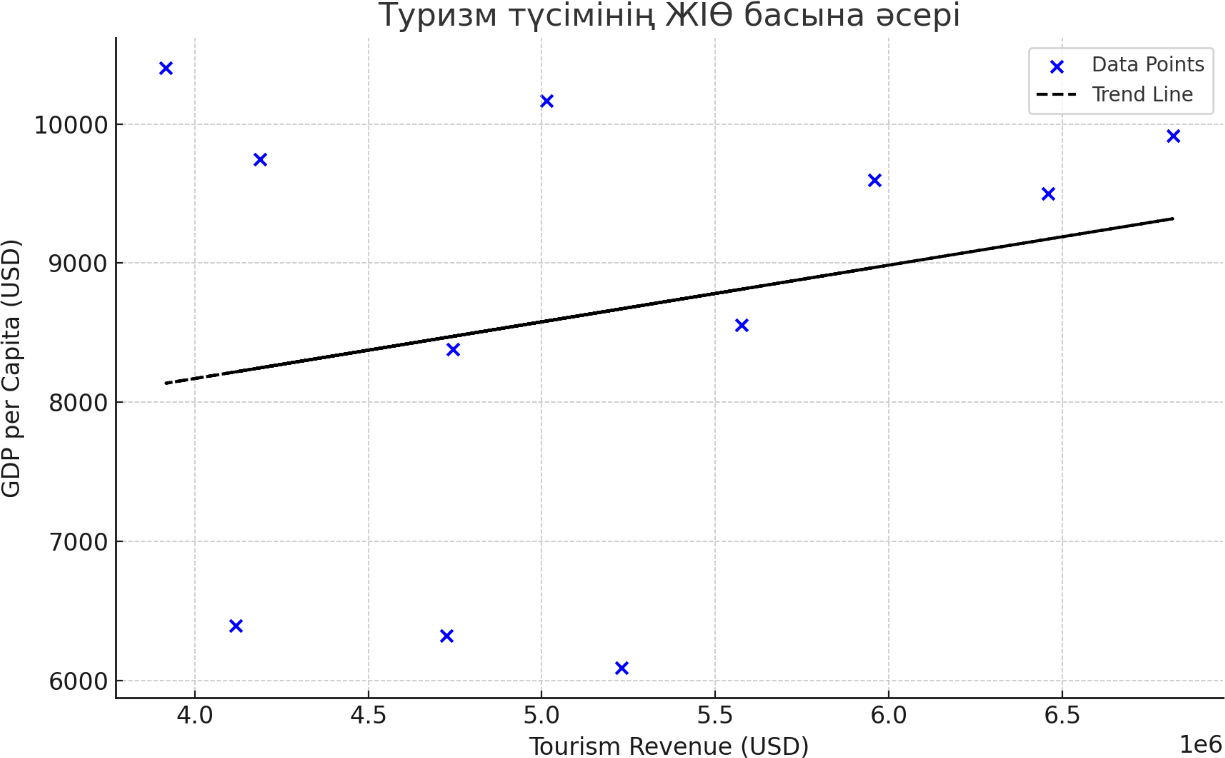
\includegraphics[width=0.8\textwidth]{assets/1114}
	\caption*{1-сурет - Туризмнен түскен табыс жан басына шаққандағы жалпы ішкі өнімге әсері.}
	\caption*{Тренд сызығы оң қатынасты көрсетеді}
\end{figure}

\begin{figure}[H]
	\centering
	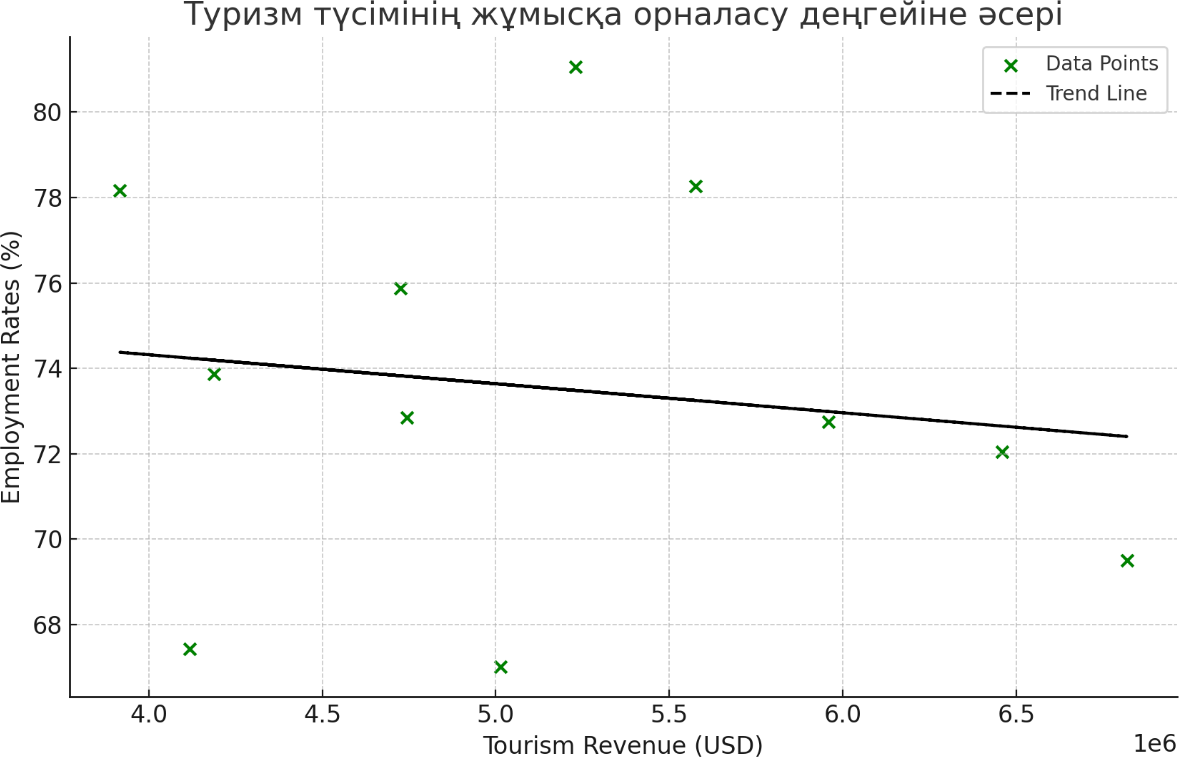
\includegraphics[width=0.8\textwidth]{assets/1115}
	\caption*{2-сурет - Туризмнен түскен табыс пен жұмыспен қамту деңгейі арасындағы корреляцияны көрсетеді}
\end{figure}

\begin{figure}[H]
	\centering
	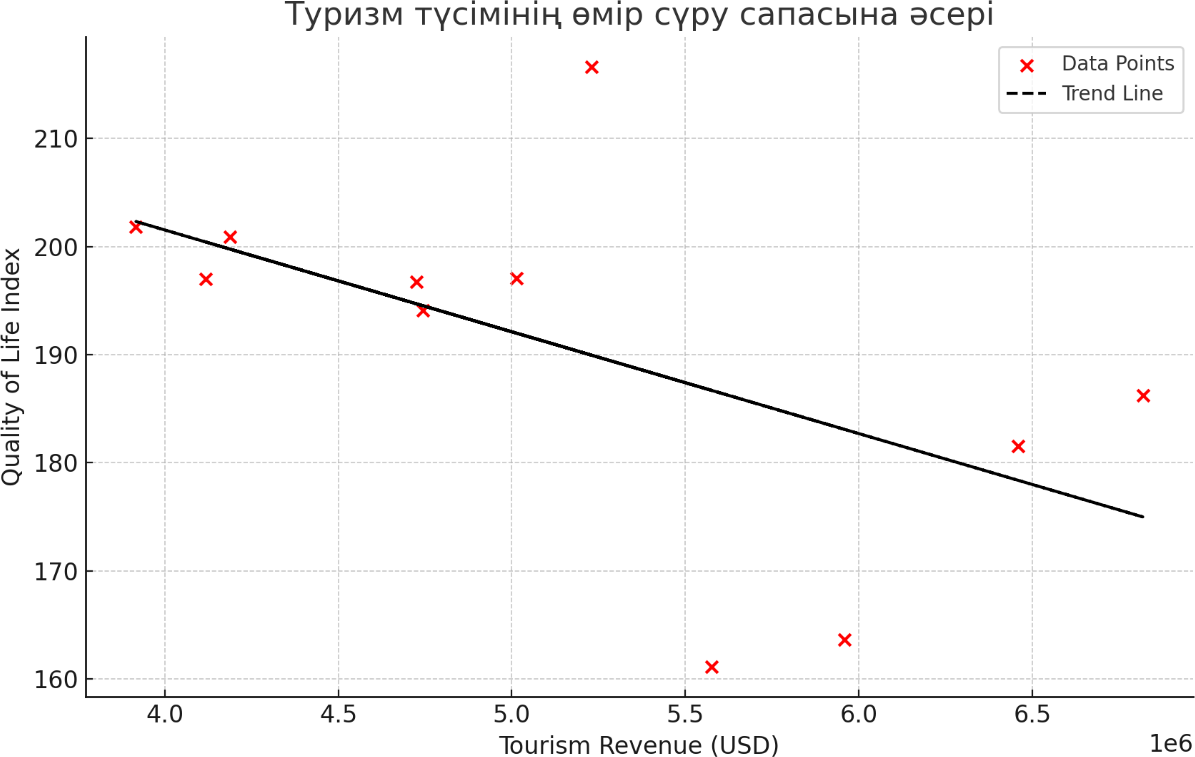
\includegraphics[width=0.8\textwidth]{assets/1116}
	\caption*{3-сурет - Туризм кірісінің артуы өмір сапасы индексін қалай жақсартуы мүмкін екенін көрсетеді}
\end{figure}

\begin{multicols}{2}
Нәтижелер туризмнен түскен табыс пен барлық үш тәуелді айнымалы
арасындағы оң және статистикалық маңызды қатынасты көрсетеді. Атап
айтқанда, туризмнен түсетін кірістің артуы жан басына шаққандағы ЖІӨ-нің
жоғарылауымен, жұмыспен қамту деңгейінің жақсаруымен және өмір сапасының
жақсаруымен байланысты.

Сұхбаттардың сапалы деректері осы тұжырымдарды толықтырады, бұл
туризмнің экономикалық тұрақтылықты нығайтып қана қоймай, сонымен қатар,
аймақтағы әлеуметтік және мәдени серпінділікке ықпал еткенін көрсетеді.

Зерттеу құнды түсініктер бергенімен, сыртқы жаһандық экономикалық
факторлардың, соның ішінде COVID-19 пандемиясының әсері сияқты
шектеулерді мойындайды. Туризмнің ұзақ мерзімді қоршаған ортаға әсерін
зерттеу және ағымдағы өсудің тұрақтылығын бағалау үшін қосымша
зерттеулер қажет.

Бұл зерттеу Солтүстік Қазақстанның әлеуметтік-экономикалық негізін
жақсартудағы туризмнің маңызды рөлін көрсетеді. Қорытындылар экологиялық
және әлеуметтік салдарларды ескере отырып, туризмнің пайдасын барынша
арттыруға бағытталған саяси шешімдерді басшылыққа алады деп күтілуде.

Қазіргі таңда Солтүстік Қазақстанның 2010-2020 жылдардағы деректерін
талдау туризмнен түскен кірістің өңір экономикасына, жұмыспен қамтуға
және өмір сүру сапасына оң әсерін айқын көрсетеді. Туризмнен түскен
табыстың артуымен жан басына шаққандағы ЖІӨ және жұмыспен қамту деңгейі
де өседі, бұл туризмнің жұмыс орындарын құруға ықпал ететін маңызды
экономикалық драйвер екенін көрсетеді. Сонымен қатар, өмір сапасы
көрсеткіштерінің жақсаруы туризмнің пайдасы экономикалық шаралардан,
инфрақұрылым мен мемлекеттік қызметтерді жақсартудан тыс екенін
көрсетеді.

Жергілікті мүдделі тараптармен жүргізілген сұхбаттар туризмнің артуына
байланысты қауымдастықтың инфрақұрылымы мен мәдени алмасудағы көрінетін
жақсартуларды атап көрсете отырып, осы тұжырымдарды растайды. Дегенмен,
зерттеу шектеулерді, соның ішінде деректерді бұрмалауы мүмкін COVID-19
пандемиясы сияқты жаһандық оқиғалардың әсерін мойындайды. Туризмнің ұзақ
мерзімді тұрақтылығын және оның қоршаған ортаға әсерін зерттеу үшін
болашақ зерттеулер ұсынылады.

Бұл зерттеу саясаткерлерге туризмді аймақтық дамудың стратегиялық
элементі ретінде пайдалану үшін негіз болып табылады, экономикалық пайда
мен тұрақтылықты теңестіреді.

{\bfseries Қорытынды.} Күрделі жүйелердің жұмыс істеу процесстерін қатаң
аналитикалық зерттеу тіпті де мүмкін емес. Олардың аналитикалық
моделдерін анықтау көптеген жағдайларға, жұмыс ерекшеліктеріне, оны
құрайтын бөліктердің өзара әрекеттеріне қара, қоршаған әсерлерге және
т.с.с байланысты қиын болып келеді. Зерттеу нәтижесінде туризмнен
түсетін табыс Солтүстік Қазақстанның әлеуметтік-экономикалық дамуына
айтарлықтай үлес қосатынын дәлелдеді. 2010 жылдан 2020 жылға дейінгі
деректерді талдайтын көп нұсқалы регрессиялық модель арқылы туристік
кірістің өсуі жан басына шаққандағы ЖІӨ-нің жоғарылауымен, жұмыспен
қамту деңгейінің жақсаруымен және өмір сапасының жақсаруымен оң
байланысты екені анық. Бұл тұжырымдар туризмнің экономикалық серпіліс
ретінде ғана емес, сонымен қатар, инфрақұрылымды дамыту мен кеңейтілген
мемлекеттік қызметтерді қоса алғанда, кең әлеуметтік игіліктер үшін
катализатор ретіндегі шешуші рөлін атап көрсетеді.

Оң нәтижелерге қарамастан, зерттеу өсу стимуляторы ретінде туризмнің
сенімділігіне әсер етуі мүмкін сыртқы экономикалық күйзеліс, әсіресе
COVID-19 пандемиясы сияқты ықтимал шектеулерді мойындайды. Осылайша,
туризмнің тікелей пайдасы анық болғанымен, оның ұзақ мерзімді
тұрақтылығы мен әсері, әсіресе қоршаған ортаға әсер ету және
экономикалық тұрақтылық салаларында қосымша зерттеулерді қажет етеді.

Осы тұжырымдарды ескере отырып, саясаткерлерге тек экономикалық өсуді
ғана емес, сонымен қатар, қоршаған орта мен мәдени құндылықтарды
сақтайтын тұрақты тәжірибеге басымдық беретін туризмге стратегиялық
инвестицияларды қарастыру ұсынылады. Бұл тәсіл Солтүстік Қазақстандағы
туризмнің гүлденген, жан-жақты және тұрақты болашаққа үлес қоса отырып,
дамудың сенімді драйвері болып қалуын қамтамасыз етеді.
\end{multicols}

\begin{center}
{\bfseries Әдебиеттер}
\end{center}

\begin{noparindent}
1. Gössling S., Scott D., Hall C. M. Pandemics, tourism and global
change: a rapid assessment of COVID-19// Journal of Sustainable Tourism.
-2020. -Vol.29(1). -P. 1-20. DOI 10.1080/09669582.2020.1758708

2. Li Y., Hu C., Huang C., Duan, L. The concept of smart tourism in the
context of tourism information services// Tourism Management. -2019.
-Vol. 58. -P. 293-300. DOI 10.1016/j.tourman.2016.03.014

3.Sigala M. New technologies in tourism: From multi-disciplinary to
anti-disciplinary advances and trajectories// Tourism Management
Perspectives. -2018. -Vol. 25. - P. 151-155. DOI
10.1016/j.tmp.2017.12.003

4.Budeanu A., Miller G., Moscardo G., Ooi C. S. (2016). Sustainable
tourism, progress, challenges and opportunities: an introduction//
Journal of Cleaner Production. -2016. -Vol. 111. -P. 285-294. DOI
10.1016/j.jclepro.2015.10.027

5.Higgins-Desbiolles F. Socialising tourism for social and ecological
justice after COVID-19. //Tourism Geographies. -2018. -Vol. 22(3). - P.
610-623. DOI 10.1080/14616688.2020.1757748

6.Brida J. G., Cortes-Jimenez I., Pulina M. Has the tourism-led growth
hypothesis been validated? A literature review. //Current Issues in
Tourism. -2016. -Vol. 19(5). - P.394-430. DOI
10.1080/13683500.2013.868414

7.Butler R. W. The concept of a tourist area cycle of evolution:
Implications for management of resources// Canadian Geographer. -1980.
-Vol. 24(1). -P. 5-12. DOI 10.1111/j.1541-0064.1980.tb00970.x

8.Kazakhstan National Statistics Office. Annual Economic Report. -2021.
--URL: https://stat.gov.kz/en/region/sko/ (date of the application
21.02.2024)

9.Local Government of North Kazakhstan. Annual Infrastructure
Development Report. -2020. --URL:

https://www.gov.kz/memleket/entities/sko/activities/4973?lang=en. (date
of the application -- 21.02.2024)

10.Kazakhstan Department of Health and Education. Social Metrics Report.
-2019. --URL:

https://www.gov.kz/memleket/entities/dsm?lang=en. (date of
the application 25.02.2024)

11.Ministry of Education and Science of the Republic of Kazakhstan.
Ethical Guidelines for Research. -2018. --URL:
https://www.gov.kz/memleket/entities/edu?lang=en. (date of the
application 26.02.2024)

12. SPSS-tі zhelіde tegіn paidalana alamyn ba?: REVIEWS. -URL:
https://reviews.tn/kk/wiki/can-i-use-spss-online-for-free/ (date of the
application -- 03.003.2024) {[}in Kazakh{]}
\end{noparindent}

\emph{{\bfseries Авторлар туралы мәліметтер}}

\begin{noparindent}
Бидахмет Ж. -PhD, әл-Фараби атындағы Қазақ ұлттық университетінің доцент
м.а., Алматы, Қазақстан,

е-mail: bidakhmetzhanar@gmail.com;

Исаев А.Р.-әл-Фараби атындағы Қазақ ұлттық университетінің
магистранты,Алматы, Қазақстан, е-mail: aydarisaev@mail.ru
\end{noparindent}

\emph{{\bfseries Infоrmatiоn abоut the authоrs}}

\begin{noparindent}
Zh. Bidakhmet -- PhD, аcting Associate professor Al-Farabi Kazakh
National University, Almaty, Kazakhstan,

е-mail: bidakhmetzhanar@gmail.com;

A. Issayev- graduate student at Al-Farabi Kazakh National University,
Almaty, Kazakhstan ,е-mail: aydarisaev@mail.ru
\end{noparindent}
